% This is samplepaper.tex, a sample chapter demonstrating the
% LLNCS macro package for Springer Computer Science proceedings;
% Version 2.21 of 2022/01/12
%
\documentclass[runningheads]{llncs}
%loke
\usepackage[T1]{fontenc}
% T1 fonts will be used to generate the final print and online PDFs,
% so please use T1 fonts in your manuscript whenever possible.
% Other font encondings may result in incorrect characters.
%
\usepackage{graphicx}
\usepackage{tikz}
\usepackage{pgfplots}
\usepackage{bchart}
\usepackage{rotating} % <-- HERE
\usepackage{float}
\usepackage{lscape}
\usepackage{hyperref}
\usepackage[verbose]{placeins}
\usetikzlibrary{shapes, arrows}
% remove title on each page
% \pagestyle{plain}
\usepackage{fancyhdr}
\pagestyle{fancy}
\fancyhf{}
\fancyhf[rh]{\thepage}% right header
\renewcommand\headrulewidth{0pt}% remove if you want a rule beneath the header
% \fancyhf{}
% \fancyhead[LE,RO]{}
% \fancyhead[LO,RE]{}
% \fancyfoot[CE,CO]{}
% \fancyfoot[LE,RO]{}
% \setlength{\headheight}{15pt}

\makeatletter
\newdimen\legendxshift
\newdimen\legendyshift
\newcount\legendlines
% distance of frame to legend lines
\newcommand{\bclldist}{1mm}
\newcommand{\bclegend}[3][10mm]{%
    % initialize
    \legendxshift=0pt\relax
    \legendyshift=0pt\relax
    \xdef\legendnodes{}%
    % get width of longest text and number of lines
    \foreach \lcolor/\ltext [count=\ll from 1] in {#3}%
        {\global\legendlines\ll\pgftext{\setbox0\hbox{\bcfontstyle\ltext}\ifdim\wd0>\legendxshift\global\legendxshift\wd0\fi}}%
    % calculate xshift for legend; \bcwidth: from bchart package; \bclldist: from node frame, inner sep=\bclldist (see below)
    % \@tempdima: half width of bar; 0.72em: inner sep from text nodes with some manual adjustment
    \@tempdima#1\@tempdima0.5\@tempdima
    \pgftext{\bcfontstyle\global\legendxshift\dimexpr\bcwidth-\legendxshift-\bclldist-\@tempdima-0.72em}
    % calculate yshift; 5mm: heigt of bar
    \legendyshift\dimexpr5mm+#2\relax
    \legendyshift\legendlines\legendyshift
    % \bcpos-2.5mm: from bchart package; \bclldist: from node frame, inner sep=\bclldist (see below)
    \global\legendyshift\dimexpr\bcpos-2.5mm+\bclldist+\legendyshift
    % draw the legend
    \begin{scope}[shift={(\legendxshift,\legendyshift)}]
    \coordinate (lp) at (0,0);
    \foreach \lcolor/\ltext [count=\ll from 1] in {#3}%
    {
        \node[anchor=north, minimum width=#1, minimum height=5mm,fill=\lcolor] (lb\ll) at (lp) {};
        \node[anchor=west] (l\ll) at (lb\ll.east) {\bcfontstyle\ltext};
        \coordinate (lp) at ($(lp)-(0,5mm+#2)$);
        \xdef\legendnodes{\legendnodes (lb\ll)(l\ll)}
    }
    % draw the frame
    \node[draw, inner sep=\bclldist,fit=\legendnodes] (frame) {};
    \end{scope}
}
% Used for displaying a sample figure. If possible, figure files should
% be included in EPS format.
%
% If you use the hyperref package, please uncomment the following two lines
% to display URLs in blue roman font according to Springer's eBook style:
%\usepackage{color}
%\renewcommand\UrlFont{\color{blue}\rmfamily}
%
\begin{document}
%
\title{Human Resource Allocation Strategy: A Systematic Literature Review}
% \thanks{Supported by organization x.}}
%
%\titlerunning{Abbreviated paper title}
% If the paper title is too long for the running head, you can set
% an abbreviated paper title here
%
\author{Qichen Liu}

% \inst{1}
% \orcidID{0000-1111-2222-3333} \and
% Second Author\inst{2,3}\orcidID{1111-2222-3333-4444} \and
% Third Author\inst{3}\orcidID{2222--3333-4444-5555}}
%
% \authorrunning{F. Author et al.}
% First names are abbreviated in the running head.
% If there are more than two authors, 'et al.' is used.
%
\institute{The Technical University of Munich, Arcisstraße 21, 80333, Germany
\email{qichen.liu@tum.de}}
\maketitle              % typeset the header of the contribution
%

\begin{abstract}
Human resources have always been recognized as one of the most valuable assets within any organization. Efficiently managing and allocating human resources is crucial to minimize monetary and time costs while simultaneously enhancing overall performance. Researchers have explored numerous approaches to achieve these objectives. Different software applications, mathematical models, and algorithms have been discussed and implemented. 
\keywords{Human resource \and Resource allocation in business process}
\end{abstract}
%
%
%
\section{Introduction}
In an organization, there are two essential components: the people who work there and the physical assets and resources it has. Employees are spread across various departments, each possessing unique skill sets and levels of experience. Additionally, different tasks vary in terms of their priority, importance, and complexity, requiring specific knowledge and different amounts of time to complete. As a result, it becomes crucial for employers and managers to allocate the appropriate human resources to carry out the respective tasks.
\\
In recent years, there has been a surge in the development of approaches aimed at enhancing human resource allocation. Their objective extends beyond reducing time and monetary costs to encompass various other factors such as synergy value, allocation accuracy, material occupancy, skill coverage rate, and ergonomic burden. In contrast to the traditional manual and informal human allocation process, these proposed approaches embrace a more formalized methodology. They employ proper mathematical models, calculations, supportive software, and algorithmic pseudo code, enabling human resource allocation to be carried out in a formal, reproducible, and effective manner.
\\
The multitude of approaches and techniques available offers a systematic perspective on the current state and advancements in human resource allocation strategies. This comprehensive view can guide managers and employers in selecting the appropriate method for their specific scenarios and requirements. While existing studies and literature reviews on resource allocation in business processes primarily focus on material resource management or resource allocation in general, they do not delve into the intricacies of human resource allocation. While these resources may provide some insights, they may not fully address real-life human resource allocation challenges. Hence, this study aims to bridge this research gap by providing a detailed examination of human resource allocation strategies. It discusses recent trends, developed techniques, algorithms, and their enhancements, while categorizing them based on different criteria. This work follows a rigorous and replicable systematic literature review (SLR) methodology, as specified by Kitchenham.
\\
In the remainder of this paper, the research question I want to investigate are given in Section 2 and the process of identifying relevant researches as well as SLR protocol are explained in Section 3. Section shows how information was extracted from studies. In section 5, we go through all the research questions and give present answers to them respectively.

\section{Research Questions}
This study aims to provide a detailed understanding of the current state and development of human resource allocation strategies. To achieve this, the research will be structured by addressing several specific subquestions, allowing for an organized and systematic investigation.\\
\begin{itemize}
    \item RQ1 What are the recent trends in human resource allocation study?\\
    The goal of this research question is to discover new ideas and aspects of human resource allocation in the past 2 years.By investigating the reasons behind popularity of certain methodologies, we can gain a better understanding of human resource allocation and business processes.\\
    \item RQ2 What algorithms and techniques have been proposed and developed in recent years?\\
    Examining the concrete techniques in human resource allocation provides valuable insights into bridging the gap between theoretical ideas and practical implementation. This analysis is crucial for understanding how human resource allocation processes are actually carried out by studying the usage of the techniques in real-life examples, including simulations and experiments. This understanding equips managers and employers with examples that they can adopt or adapt to develop their own strategies.\\
    \item RQ3 What improvements do these approaches offer in terms of cost, time or other aspects?\\
    With this research question, the focus is on understanding the improvements provided by the proposed approaches, particularly in a statistical form. Additionally, it is interesting to explore the other improvement indicators that are considered. By analyzing the relationship between these statistics and other attributes of the approaches, such as maturity and application domain, we can gain insights into what constitutes a successful strategy. This analysis provides valuable guidance for future research in the field of human resource allocation.
\end{itemize} 


\section{Identifying relevant studies}
\subsection{Search process}
To identify relevant studies, a two-phase search approach was employed, consisting of a primary search and a secondary search. During the primary search, high-trust research databases were queried using predefined search terms. This initial search yielded a substantial number of studies, forming a preliminary set of works. From these studies, information such as title, abstract, and other relevant details were extracted into a .csv file. A core set of papers was then selected by carefully reviewing their titles, abstracts, and publication year. Initially, the focus was on journal articles due to the extensive number of conference papers and proceedings available. As a result of the primary search, 10 journal papers were identified. It is important to note that this search was conducted in June 2023.
\\
During the primary search, two trusted databases, IEEE Xplore and ACM Digital Library, were queried. A total of 536 journal articles were found across these databases. The specific search queries used for each database can be found in table below.


% \begin{center}
\begin{figure}
% \begin{table}
% \caption{Table captions should be placed above the
% tables.}\label{tab1}
\scalebox{0.52}{
\begin{tabular}{||c c c||} 
 \hline
 Database & Search queries & Number \\ [0.5ex] 
 \hline\hline
 IEEE Xplore & ((human resource OR task OR staff OR resource) AND (allocation OR assignment OR scheduling OR optimization OR planning)) & 418\\ 
 \hline
 ACM Digital Library & Abstract:((human resource staff task) AND (allocation assignment scheduling optimization planning) & 118 \\

  \hline
\end{tabular}
}
\caption{Database, search queries, and resulting number of studies in the primary search.}
\end{figure}
% \end{table}
% \end{center}
\noindent
In the secondary search, a forward and backward search was conducted to primarily include more relevant conference papers, thereby maximizing the completeness of the search. Upon reviewing several conference papers, it was observed that many of them exhibited high quality and maturity or provided intriguing aspects, particularly in terms of the improvements offered by the proposed approaches. As a result, an additional 19 conference studies were identified and added to the core set, bringing the total number of studies to 29.
The complete search process with the resulting numbers of studies is illustrated in the flow chart below.\\

\begin{figure}[H]
\tikzstyle{process} = [rectangle, 
minimum width=0.5cm, 
minimum height=0.5cm, 
text centered, 
scale = 1,
text width=0.5cm, 
draw=black, 
fill=white!30]

\begin{tikzpicture}[node distance=2cm]

\node (pro2b) [process, xshift=1.8cm] {536};
\node (pro2c) [process, right of=pro2b, xshift=1.8cm] {10};
\node (pro2d) [process, right of=pro2c, xshift=1.8cm] {29};
\node (pro2e) [process, right of=pro2d, xshift=1.8cm] {19};


\draw [->] (pro2b) -- (pro2c) node[midway, above, align=center] {Read titles\\and abstracts};
\draw [->] (pro2c) -- (pro2d) node[midway, above, align=center] {In forward \& backward\\search, 19 conference\\papers were found};
\draw [->] (pro2d) -- (pro2e) node[midway, above, align=center] {10 papers were\\excluded due to low \\quality/irrelevancy};;

\end{tikzpicture}
\caption{Search process and the number of studies as result of the difference steps.}
\end{figure}


\subsection{Criteria}
Here are the inclusion and exclusion criteria used to guide the selection of studies during the search process:
\begin{itemize}
    \item IN1 The study (i)describes an approach/algorithm that supports human resource allocation in business process and (ii)was published within the last 2 years.

    \item EX1 The study primarily focus on material/vehicle resource allocation
    \item EX2 The study does not include any of the following aspects in human resource allocation strategy: 
    \begin{itemize}
        \item A real-life experiment of the approach with detailed documentation
        \item A artificial simulation of the approach with detailed documentation
        \item Pseudo code of the allocation algorithm
    \end{itemize}
\end{itemize}
Inclusion criterion "Studies merely introduce a flow chart of the general methodology" was abandoned due to the low quality of such works.

\section{Data extraction}
After thoroughly reviewing the final set of 29 studies, an additional 10 studies were excluded. These exclusions were based on the fact that the studies were either (i) not directly relevant to the topic or (ii) of insufficient quality or maturity level.  \\The relevant information was extracted according to the following predefined data scheme:
\begin{itemize}
    \item Country, Year
    \item Application domain
    \item Technique
    \item Improvement
    \item Maturity
\end{itemize}

\begin{figure}[H]
\scalebox{0.7}{
\begin{bchart}[steps={2, 4, 6, 8, 10},max=10]
\bcbar[label=China]{8} \bcskip{5pt}
\bcbar[label=Italy]{2} \bcskip{5pt}
\bcbar[label=UK]{1} \bcskip{5pt}
\bcbar[label=Korea]{1} \bcskip{5pt}
\bcbar[label=Iran]{1} \bcskip{5pt}
\bcbar[label=Slovenia]{1} \bcskip{5pt}
\bcbar[label=Philippines]{1} \bcskip{5pt}
\bcbar[label=India]{1} \bcskip{5pt}
\bcbar[label=Brazil]{1} \bcskip{5pt}
\bcbar[label=Morocco]{1} \bcskip{5pt}
\bcbar[label=US]{1} \bcskip{5pt}
\bcxlabel{Originating Country}
\end{bchart}
}
\end{figure}

\noindent
In the upcoming sections where the research questions are addressed, additional extracted data will be presented, providing further insights and evidence related to the research topic.

\begin{sidewaystable} % <-- HERE
\centering
\begin{tabular}{cccccccc}\hline
Reference & Year & Country & Application domain & Technique & Improvement & Maturity\\\hline
Arindam Roy et al.\cite{study10} & 2021 & India & General & Software(Python) & Not specified & Medium\\

YUE CUI.\cite{study12} & 2021 & China & General & Improved ant colony algo. & Balance, efficiency & Medium\\

Sufen Jiang.\cite{study13} & 2021 & China & General & Linear programming & Not specified & Low\\

Yang Jiao.\cite{study14} & 2021 & China & General & Math model, genetic algo. & Not clearly explained & Low\\

XueJie Bai et al.\cite{study15} & 2021 & China & Rural e-commerce & Big data mining and analysis & Accuracy, rationality & Medium\\

Augusto Urru et al.\cite{study16} & 2021 & Germany & Shifting & Math model & Not specified & Low \\

SiChong Ma et al.\cite{study17} & 2021 & China & General & Genetic algo. & Not specified & Low\\

Miljenko Hajnić et al.\cite{study18} & 2021 & Slovenia & Employee transferring & Software: Web System & Time, cost & High\\

Jiuchuan Jian.\cite{study19} & 2021 & China & General & Software(Java) & Synergy, conflicts, skill coverage & Medium &\\
Davide La Torre et al\cite{study2} & 2021 & Italy & General & GP \& num. analysis & Not specified & Medium\\


Chenxiang Ma et al.\cite{study3} & 2022 & China & General & Decision tree & Not specified & Low\\

Omid Mahdi Ebadati et al.\cite{study4}& 2022 & Iran & Banking industry & Process mining, Software & Solve bottleneck & Medium\\

Na Feng.\cite{study5} & 2022 & China & General & Decision tree & Time, cost & Medium\\

Marielle A. Cantara et al.\cite{study6} & 2022 & Philippines & City engineering office & Software, analysis & Not specified & Medium\\

Saeed Akba et al.\cite{study7} & 2022 & China \& UK & General & Software(Python) & Not specified & Medium\\

Jair José Ferronato et al.\cite{study8} & 2022 & Brazil & Hospital & Genetic Algo., Python program & Occupancy, Surgery number  & Medium & \\

Abderrahmane Benkacem et al.\cite{study9} & 2022 & Morocco & Disaster situation & Machine Learning & Not specified & Low \\

Qiaoyin Peng.\cite{study10} & 2022 & China & General & Software(Java) & Not specified & Low \\

Moon-Sook Yeon.\cite{study11} & 2022 & Korea & Ticketing management & Event logs mining & Not specified & Medium\\
Simone Guarin et al.\cite{study1} & 2023 & Italy & Network maintenance & Software & Fault cost & High\\


\hline
\end{tabular}
\caption{Studies and their categorizations ordered by publication year.}
\end{sidewaystable} % <-- HERE



\section{Human Resource Allocation Approaches}
This section presents the findings of the systematic literature review (SLR) in relation to the research questions.\\
The recent trends in human resource allocation is addressed in section 4.1. The approaches and techniques proposed are presented in section 4.2, addressing RQ2. Finally, the improvements each approach brings is discussed in section 4.3, addressing section RQ3.

\subsection{RQ1: Recent trends in human resource allocation}
In this subsection, we address \emph{RQ1: What are the recent trends in human resource allocation?} We explore the general ideas and methodologies behind these trends, focusing on understanding the overarching concepts in the literature.
\subsubsection{Solutions to specific application domain} Recent studies tend to provide a solution which applies to a specific rather than just approaches that fits in general situations. \\
For example, in study \cite{study1}, the authors recognize that Critical infrastructures (CI) are physical infrastructures essential for the efficiency, security and the correct functioning of a nation. Thus they investigate specifically in network maintenance crew dispatching and conducted simulation in city Rome. \\
Study\cite{study9} utilizes machine learning with the aim of optimizing human resource allocation under disaster situations. In such situations, a large number of patients may be generated at one time, potentially exceeding the capacity of available resources.\\
Approaches for other specific scenarios are discussed including rural e-commerce\cite{study15}, banking industry\cite{study4}, city engineering office \cite{study6} and ticketing management\cite{study11}.

\subsubsection{Investigating in human networks}
Some studies go beyond considering human resources as separate individuals and instead focus on exploring the network and social relationships among personnel. They recognize that employees often form naturally organized groups. Therefore, finding effective solutions for assigning human resources to groups and dispatching these groups to the appropriate tasks based on their skill sets and experience becomes crucial. This approach takes into account the collective dynamics and interactions among employees, leading to more efficient and optimized human resource allocation strategies.\\
For example, in study \cite{study19}, the authors focus on 2 main problems: (i) measuring the priority of a group being allocated a task by considering its contextual groups and (ii) examining how an assigned group coordinates with other contextual groups during task performance. The study introduces a metric called contextual crowdsourcing value, which asseses a group's capacity to perform a task by coordinating with its contextual groups. Additionally, a method for modeling group coordination in task performance is presented. The study categorizes groups into 2 types: Group with Leaders, Group without Leaders, and provides algorithms for selection of workers within groups as well as allocating groups.\\
Another example, Study \cite{study2}, while not extensively considering the social network between employees, still emphasizes the importance of teams over individuals. The study employs multi-criteria decision making and goal programming to develop a model that assists managers in forming cost-effective teams with high levels of trust. By utilizing these methodologies, the study aims to enhance the group formation process within organizations.\\
In Study \cite{study11}, the authors explore the concept of human-centric networks within an organization by mining its operational event log history. By analyzing and comprehending the holistic perspectives of the operational process as provided by these networks, managers gain clarity on the probabilities of appropriateness for allocating employees to each activity. The study also considers centrality metrics of employees within the networks in various aspects. This comprehensive understanding enables managers to effectively allocate resources for the subsequent operations of the enterprise.\\
In summary, analyzing personnel in groups and their networks provides managers with a comprehensive overview of human resources, facilitating better allocation decisions.
\subsubsection{Focuses other than time/money cost}
Many studies follow the traditional evaluation scheme of human resource allocation, namely aiming at reduce the time and monetary cost of the business process. However, a few studies reviewed by this work also concerns some other interesting and valuable aspects, which are shown below:
\begin{itemize}
    \item Synergy value
    \item Accuracy
    \item Rationality
    \item Occupancy
    \item Balance
    \item Skill coverage rate
    \item Ergonomic Burden
\end{itemize}
For instance, the paper \cite{study16} addresses the issue of ergonomic burden. It introduces a method to monitor the actual ergonomic burden experienced by resources during a shift and proposes a linear optimization model to guide the resource allocation process. The study particularly emphasizes dynamic logistics environments, where the cumulative ergonomic burden on a single human resource throughout a shift may be unpredictable. To ensure fair working conditions, monitoring the evolution of ergonomic burden becomes essential.\\
In \cite{study8}, the author discusses resource allocation in hospitals during emergency situations, specifically focusing on operating room scheduling and surgeon allocation. The proposed method aims to enhance the operating room occupancy rate and increase the number of surgeries performed under various circumstances.\\
While \cite{study15} addresses the concept of allocation rationality, \cite{study19} aims to enhance synergy value and consistency etc. in resource allocation.
\begin{figure}
\scalebox{1}{
\begin{bchart}[steps={2, 4, 6, 8, 10, 12, 14},max=14]
\bcbar[label=Time]{4} \bcskip{5pt}
\bcbar[label=Cost]{3} \bcskip{5pt}
\bcbar[label=Others]{12} \bcskip{2pt}
\bcxlabel{Distribution of Improvement Aspects in Studies}
\end{bchart}
}
\end{figure}


\subsection{RQ2: Approaches and techniques}
In this subsection, we investigate \emph{RQ2: What algorithms and techniques have been proposed developed in recent years?} By examining the technical details and practical applications of these approaches, organizers can gain inspiration for developing their own human resource allocation strategies that align with their specific requirements and organizational contexts.\\
The techniques proposed in the reviewed studies can be broadly categorized into two types based on their maturity levels and goals: computer software and mathematical models/algorithms.\\
Furthermore, the reviewed studies employed various types of experiments and simulations, which served as verification measures, to assess the applicability and feasibility of the proposed methods and techniques. \\
\begin{figure}
\scalebox{0.9}{
\begin{bchart}[steps={0, 5, 10, 15, 20},max=20]
\bcbar[label=Computer Software]{9} \bcskip{5pt}
\bcbar[label=Math model]{19} \bcskip{5pt}
\bcbar[label=Pseudo code]{5} \bcskip{5pt}
\bcxlabel{Categorization of proposed Techniques/Methods}
\end{bchart}
}
\end{figure}

\subsubsection{Computer Software}
For example, in \cite{study18} integrated their model into a web-based System to support a human resource transferring process with less time and operational costs. In \cite{study8}, Jair José Ferronato et al. implemented their algorithm using Python programming language to carry out experimentations on computer.
\subsubsection{Mathematical Model}
All studies proposed some kind of mathematical model to represent different factors such as resource, project number, capacity of employee etc. For example, study \cite{study15} models new function and uses mathematical analysis to calculate the information entropy that divides the rural e-commerce human resource data according to related attributes.
\subsubsection{Pseudo code of algorithm}
In study \cite{study7}, pseudo code of scheduling projects, scheduling tasks as well as assigning resources are provided. Those algorithms depict the exact steps to perform the proposed approaches in a clear and concise way.\\
\newline
\newline
Some studies conducted simulations either on artificial organizations\cite{study4,study7,study8,study13,study14,study19} or real companies\cite{study1,study11,study15,study18} as a means of verification. In contrast, other studies did not provide any form of verification, which may diminish their reliability and trustworthiness.

\subsubsection{Simulation on artificial Org}
In e.g \cite{study14}, computer simulations were conducted with different parameters, such as estimated completion time, priority weight factor, delay cost loss and workload, in order to gain a more comprehensive evalution. 
\subsubsection{Simulation on real Org}
In \cite{study5}, simulations were carried out on various entities, including an enterprise, a e-government project team as well as a campus team. In \cite{study1}, the authors examined a real scenario involving electrical distribution network of city Rome. These experiments, conducted within real organization and scenarios enhances the reliability of the conclusions.
\subsubsection{No verification}
Some studies, including \cite{study16}, did not provide any experimental or simulation-based verification. Consequently, the reliability of these works may not be considered as high as those that included such verification. However, these studies were still included and reviewed due to other valuable aspects they offered, such as introducing new improvement aspects or addressing novel research angles.\\
The diagram below illustrates the distribution of studies based on the types of simulations conducted:
\begin{figure}[H]
\scalebox{0.9}{
\begin{bchart}[steps={2, 4, 6, 8, 10, 12},max=12]
\bcbar[label=Simulation on real org]{4} \bcskip{5pt}
\bcbar[label=Simulation on artificial org]{6} \bcskip{5pt}
\bcbar[label=No simulation]{9} \bcskip{2pt}
\bcxlabel{Simulation types}
\end{bchart}
}
\end{figure}

\subsection{RQ3: Improvements}
In this section, we examine the improvements brought about by the proposed approaches in the studies. Specifically, we focus on two main aspects of improvements aspects as identified in the answer to the RQ1: (i)time cost (ii)monetary cost (iii)other aspects.
\subsubsection{Time cost reduction}
Studies \cite{study5,study7,study18} have measured reduction in time costs. For example, \cite{study18} aims to provide a better employee transferring strategy, achieving an impressive 82.69\% reduction rate in time. \cite{study7} found that 44 of 50 projects could be completed earlier using their proposed approach. Additionally, \cite{study5} reported an approximate 25\% reduction in scheduling cycle through their approaches.
\subsubsection{Monetary cost reduction}
It is notable that out of the 19 studies reviewed, only 2 studies, namely \cite{study18}  and \cite{study5}, explicitly consider monetary cost in their approaches. Study \cite{study18} claims a reduction of 87.64\% in operational costs, while \cite{study5} suggests cost savings ranging from 28\% to 35\%.
\subsubsection{Other aspects}
\begin{itemize}
    \item Ergonomic burden\\
    Despite the absence of specific statistics, Study \cite{study16} still presents a fresh perspective in human resource allocation by addressing the crucial issue of reducing employees' ergonomic burden. This aspect holds significance not only for the well-being and health of employees but also for enhancing the overall performance of the organization.
    \item Synergy value, accuracy, rationality and skill coverage rate\\
    In Study \cite{study19}, the proposed approach achieves notable results, including a 2x-3x higher synergy value, approximately 1.4x fewer conflicts, and a skill coverage rate that is around 1.8x higher. However, the study does not provide a clear explanation of what these terms exactly represent and the specific benefits they offer to organizations by utilizing the proposed methods.
    \item Occupancy\\
    Study \cite{study8} investigates in hospital environment. It reports an increase in  operating room occupancy by 10\% and 25\%, number of surgeries performed from 12 to 16 and from 11 to 18 under different circumstances.
\end{itemize}
\section{Conclusion}
This survey has provided a structured analysis of approaches for human resource allocation and management. 19 studies from various countries published within last 3 years were identified and reviewed. With this SLR, we investigated the following research questions:
\begin{itemize}
    \item RQ1 What are the recent trends in human resource allocation study?
    \item RQ2 What algorithms and techniques have been proposed and developed in recent years?
    \item RQ3 What improvements do these approaches offer in terms of cost, time or other aspects?\\
    \end{itemize}
Regarding RQ1, our analysis revealed several key findings. (1)Recent studies consider human resources not only as individuals but also as groups and teams, exploring the network and social relationships among employees. (2)More studies focus on new improvement aspects such as occupancy, skill coverage rate, and ergonomic burden, in addition to traditional metrics like time and cost. (3)There is an increasing trend of developing context-specific approaches tailored to specific scenarios, resulting in higher-quality studies.\\
Regarding RQ2, we observed that the proposed solutions in the reviewed studies can be categorized into three main types: computer software, pseudo code, and mathematical models. The computer software solutions involve the development of concrete programs using programming languages such as Python, Java, etc. Pseudo code is used to provide a high-level algorithmic representation of the proposed approach. Mathematical models encompass mathematical formulations and equations that describe the resource allocation problem and guide decision-making processes.\\
To address RQ3, we analyzed the statistics presented in the studies to assess the improvements achieved. While many studies provided specific statistical data, some did not include explicit statistics. The reported improvement metrics included percentage reductions, increased efficiencies, and comparative measures, providing valuable insights into the effectiveness of the proposed approaches.\\
Future work can focus on conducting experiments to measure newly proposed improvement aspect e.g ergonomic burden and develop improved shifting plans based on the results. Additionally, establishing a benchmarking platform can further categorize and study the connection between techniques and improvements, enabling the identification of more effective strategies for specific aspects.





% \paragraph{Sample Heading (Fourth Level)}
% The contribution should contain no more than four levels of
% headings. Table~\ref{tab1} gives a summary of all heading levels.

% \begin{table}
% \caption{Table captions should be placed above the
% tables.}\label{tab1}
% \begin{tabular}{|l|l|l|}
% \hline
% Heading level &  Example & Font size and style\\
% \hline
% Title (centered) &  {\Large\bfseries Lecture Notes} & 14 point, bold\\
% 1st-level heading &  {\large\bfseries 1 Introduction} & 12 point, bold\\
% 2nd-level heading & {\bfseries 2.1 Printing Area} & 10 point, bold\\
% 3rd-level heading & {\bfseries Run-in Heading in Bold.} Text follows & 10 point, bold\\
% 4th-level heading & {\itshape Lowest Level Heading.} Text follows & 10 point, italic\\
% \hline
% \end{tabular}
% \end{table}


% \noindent Displayed equations are centered and set on a separate
% line.
% \begin{equation}
% x + y = z
% \end{equation}
% Please try to avoid rasterized images for line-art diagrams and
% schemas. Whenever possible, use vector graphics instead (see
% Fig.~\ref{fig1}).

% \begin{figure}
% 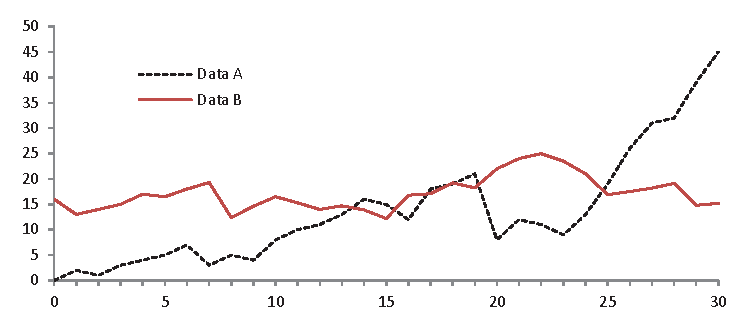
\includegraphics[width=\textwidth]{fig1.eps}
% \caption{A figure caption is always placed below the illustration.
% Please note that short captions are centered, while long ones are
% justified by the macro package automatically.} \label{fig1}
% \end{figure}

% \begin{theorem}
% This is a sample theorem. The run-in heading is set in bold, while
% the following text appears in italics. Definitions, lemmas,
% propositions, and corollaries are styled the same way.
% \end{theorem}
% %
% % the environments 'definition', 'lemma', 'proposition', 'corollary',
% % 'remark', and 'example' are defined in the LLNCS documentclass as well.
% %
% \begin{proof}
% Proofs, examples, and remarks have the initial word in italics,
% while the following text appears in normal font. 
% \end{proof}
% For citations of references, we prefer the use of square brackets
% and consecutive numbers. Citations using labels or the author/year
% convention are also acceptable. The following bibliography provides
% a sample reference list with entries for journal
% articles~\cite{ref_article1}, an LNCS chapter~\cite{ref_lncs1}, a
% book~\cite{ref_book1}, proceedings without editors~\cite{ref_proc1},
% and a homepage~\cite{ref_url1}. Multiple citations are grouped
% \cite{ref_article1,ref_lncs1,ref_book1},
% \cite{ref_article1,ref_book1,ref_proc1,ref_url1}.

% \subsubsection{Acknowledgements} Please place your acknowledgments at
% the end of the paper, preceded by an unnumbered run-in heading (i.e.
% 3rd-level heading).

%
% ---- Bibliography ----
%
% BibTeX users should specify bibliography style 'splncs04'.
% References will then be sorted and formatted in the correct style.
%
% \bibliographystyle{splncs04}
% \bibliography{mybibliography}
%
\begin{thebibliography}{8}
\bibitem{study1}
Simone Guarino, Gabriele Oliva, Antonio Di Pietro, Maurizio Pollino, Vittorio Rosato. 2023. A Spatial Decision Support System for Prioritizing Repair Interventions on Power Network. \emph{IEEE Access}
\bibitem{study2}
Davide La Torre, Cinzia Colapinto, Ilaria Durosini, Stefano Triberti. 2021. Team Formation for Human-Artificial Intelligence Collaboration in the Workplace: A Goal Programming Model to Foster Organizational Change. \emph{IEEE Transactions on Engineering Management}

\bibitem{study3}
Zahra Zahedi, Sailik Sengupta∗, Subbarao Kambhampati. 2023. ‘Why didn’t you allocate this task to them?’ Negotiation-Aware Task Allocation and Contrastive Explanation Generation Extended Abstract. \emph{AAMAS '23: Proceedings of the 2023 International Conference on Autonomous Agents and Multiagent Systems}

\bibitem{study4}
Omid Mahdi Ebadati, Mohammad Mehrabioun, Shokoofeh Hosesini. 2022. Human Resource Allocation to the Credit Requirement Process, A Process Mining Approach. \emph{2022 13th International Conference on Information and Knowledge Technology (IKT)}
\bibitem{study5}
Na Feng. 2022. Human Resource Intelligent Scheduling Algorithm Based on Decision Tree Algorithm. \emph{2022 IEEE 2nd International Conference on Mobile Networks and Wireless Communications (ICMNWC)}
\bibitem{study6}
Marielle A. Cantara, John Lhor C. Melendrez, Jason B. Tubera, Julian Robert S. Obamos, Maria Nenita S. Molinyawe, Michael M. Parondo, Jesse Ian Llyod L. Alcaraz, Sarah C. Vanguardia. 2022. Program for the Task Allocation Model: Integrating Workforce Planning for Manpower Utilization at City of Cabuyao Engineering Office\emph{TENCON 2022 - 2022 IEEE Region 10 Conference (TENCON)}
\bibitem{study7}
Saeed Akbar, Iftikhar Ahmad, Rizwan Khan, Ivandro Ortet Lopes, Rahmat Ullah. Multi-Skills Resource Constrained and Personality Traits Based Project Scheduling. 2022. \emph{IEEE Access}

\bibitem{study8}
Jair José Ferronato, Edson Emílio Scalabrin, Deborah Ribeiro Carvalho. 2022. PM4SOS: low-effort resource allocation optimization in a dynamic environment \emph{2022 IEEE International Conference on Systems, Man, and Cybernetics (SMC)}

\bibitem{study9}
Abderrahmane Benkacem, Oualid Kamach, Samir Chafik, Youness Frichi. 2022. Supervised machine learning to allocate emergency department resources in disaster situations. \emph{2022 14th International Colloquium of Logistics and Supply Chain Management (LOGISTIQUA)}

\bibitem{study10}
Arindam Roy, Shamik Sural, Arun Kumar Majumdar, Jaideep Vaidya, Vijayalakshmi Atluri. 2021. Enabling Workforce Optimization in Constrained Attribute-Based Access Control Systems. \emph{IEEE Transactions on Emerging Topics in Computing}

\bibitem{study11}
Moon-Sook Yeon, Young-Koo Lee, Dinh-Lam Pham, Kwanghoon Pio Kim. 2022. Experimental Verification on Human-Centric Network-Based Resource Allocation Approaches for Process-Aware Information Systems. \emph{IEEE Access}

\bibitem{study12}
YUE CUI. 2021. Research on dynamic allocation of human resources based on Improved Ant Colony Optimization. \emph{2021 International Conference of Social Computing and Digital Economy (ICSCDE)}

\bibitem{study13}
Sufen Jiang. 2021. An Enterprise Human Resource Allocation Management Model Based on CMMI. \emph{2021 International Conference on Intelligent Transportation, Big Data & Smart City (ICITBS)}

\bibitem{study14}
Yang Jiao. 2021. Human Resource Allocation Method Based on Multi Objective Optimization. \emph{2021 International Conference on Intelligent Transportation, Big Data & Smart City (ICITBS)}

\bibitem{study15}
XueJie Bai, Wenbei Li, Qian Zhang. 2021. Research on the optimization of rural e-commerce human resources based on big data. \emph{2021 International Conference on Intelligent Transportation, Big Data & Smart City (ICITBS)}

\bibitem{study16}
Augusto Urru, Jan Philipp Wezel, Marco Bonini, Wolfgang Echelmeyer. 2021. Dynamic Resource Allocation Considering Ergonomics in Intralogistics. \emph{2021 IEEE 25th International Conference on Intelligent Engineering Systems (INES)}

\bibitem{study17}
SiChong Ma, Shi Song Deng. Research on Software Project Scheduling Based on Genetic Algorithm. 2021. \emph{2021 IEEE 2nd International Conference on Big Data, Artificial Intelligence and Internet of Things Engineering (ICBAIE)}

\bibitem{study18}
Miljenko Hajnić, Biljana Mileva Boshkoska. A Disruptive Decision Support Platform for Reengineering the Strategic Transfer of Employees. 2021. \emph{IEEE Access}

\bibitem{study19}
Jiuchuan Jiang, Bo An, Yichuan Jiang, Chenyan Zhang, Zhan Bu, Jie Cao. 2021. Group-Oriented Task Allocating for Crowdsourcing in Social Networks. \emph{IEEE Transactions on Systems, Man, and Cybernetics: Systems}

\end{thebibliography}
\end{document}
